\documentclass[border=10pt]{standalone}
\usepackage{pgfplots}
\pgfplotsset{compat=1.18}

\definecolor{disruptor}{HTML}{2563EB}
\definecolor{aeron}{HTML}{DC2626}

\begin{document}
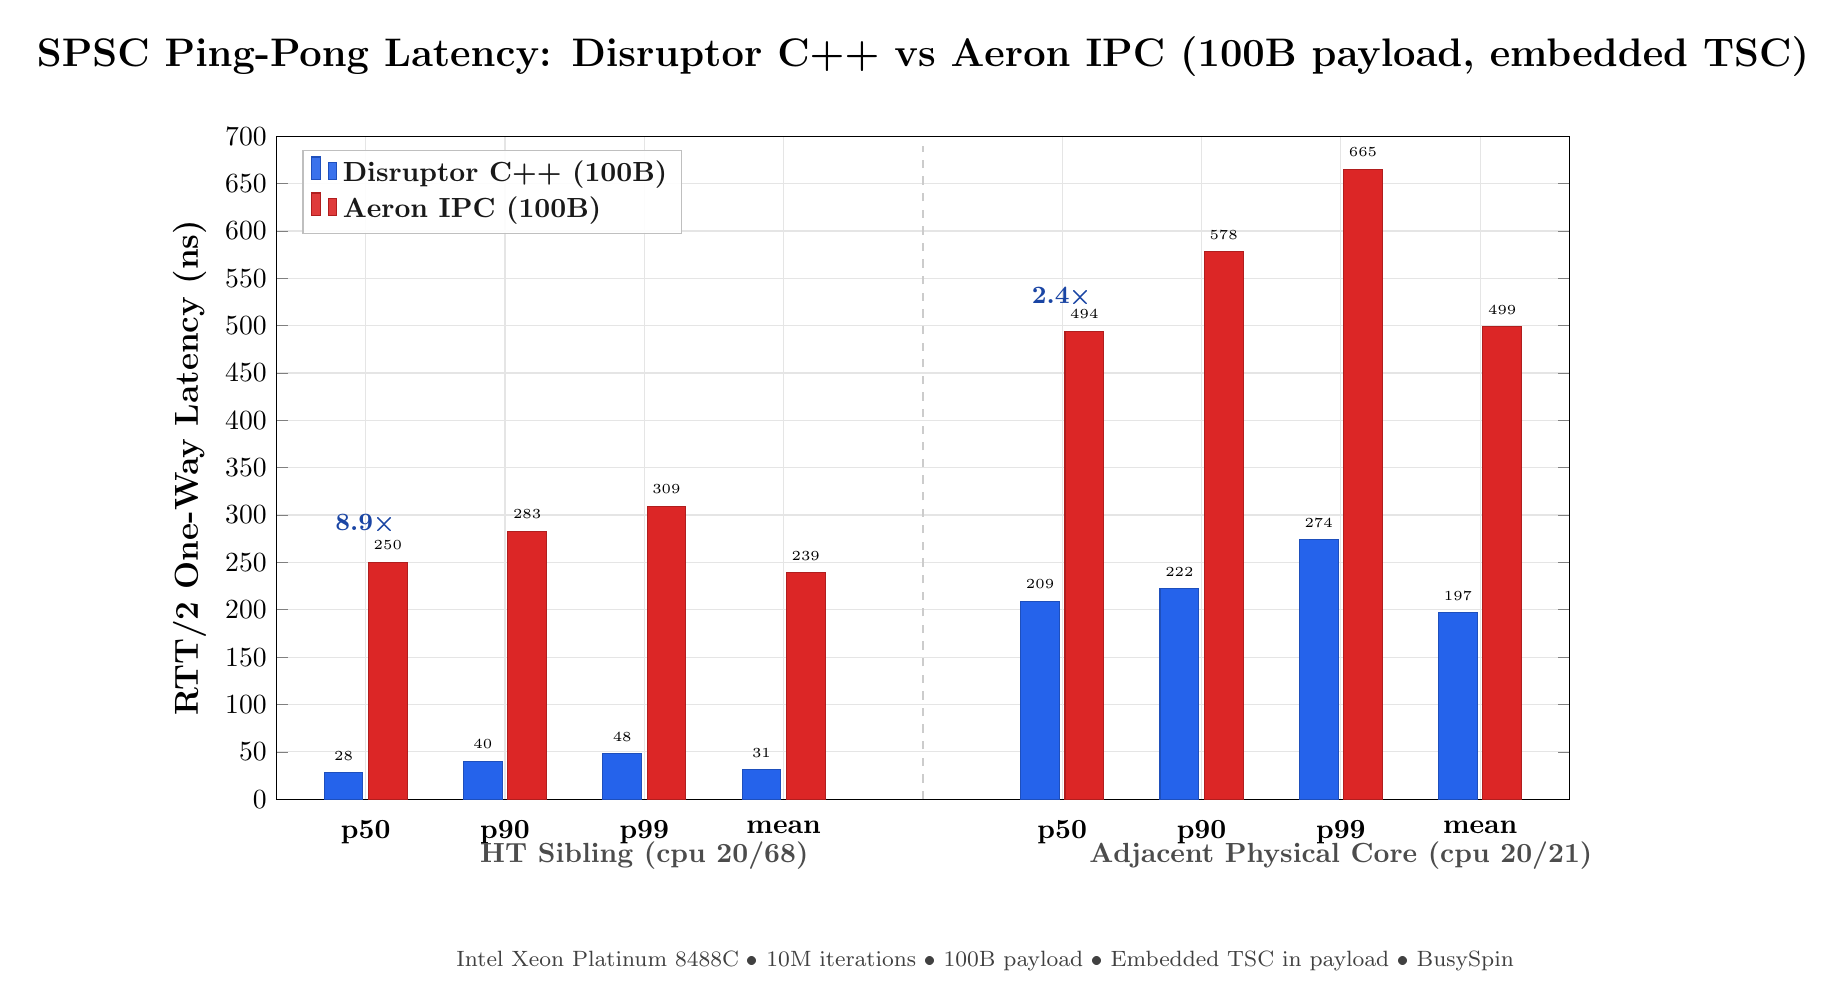
\begin{tikzpicture}
\begin{axis}[
    ybar,
    width=18cm,
    height=10cm,
    bar width=14pt,
    ylabel={RTT/2 One-Way Latency (ns)},
    ylabel style={font=\large\bfseries},
    title={\Large\bfseries SPSC Ping-Pong Latency: Disruptor C++ vs Aeron IPC (100B payload, embedded TSC)},
    title style={at={(0.5,1.05)}},
    symbolic x coords={p50a, p90a, p99a, meana, sep, p50b, p90b, p99b, meanb},
    xtick={p50a, p90a, p99a, meana, p50b, p90b, p99b, meanb},
    xticklabels={p50, p90, p99, mean, p50, p90, p99, mean},
    xticklabel style={font=\bfseries},
    ymin=0,
    ymax=700,
    ytick={0,50,100,150,200,250,300,350,400,450,500,550,600,650,700},
    nodes near coords,
    nodes near coords style={font=\tiny\bfseries, anchor=south},
    every node near coord/.append style={yshift=1pt},
    legend style={
        at={(0.02,0.98)},
        anchor=north west,
        font=\bfseries,
        draw=gray!50,
        fill=white,
        fill opacity=0.9,
    },
    legend cell align={left},
    grid=major,
    grid style={gray!20},
    major x tick style={draw=none},
    clip=false,
    enlarge x limits=0.08,
]

% Disruptor C++
\addplot[fill=disruptor, draw=disruptor!80!black] coordinates {
    (p50a, 28) (p90a, 40) (p99a, 48) (meana, 31)
    (p50b, 209) (p90b, 222) (p99b, 274) (meanb, 197)
};

% Aeron IPC
\addplot[fill=aeron, draw=aeron!80!black] coordinates {
    (p50a, 250) (p90a, 283) (p99a, 309) (meana, 239)
    (p50b, 494) (p90b, 578) (p99b, 665) (meanb, 499)
};

\legend{Disruptor C++ (100B), Aeron IPC (100B)}

% Vertical separator
\draw[dashed, gray!40, thick] (axis cs:sep, 0) -- (axis cs:sep, 690);

% Group labels
\node[font=\bfseries, text=gray!60!black] at (axis cs:p99a, -60) {HT Sibling (cpu 20/68)};
\node[font=\bfseries, text=gray!60!black] at (axis cs:p99b, -60) {Adjacent Physical Core (cpu 20/21)};

% Speedup annotations (Disruptor vs Aeron, p50)
\node[font=\small\bfseries, text=disruptor!70!black] at (axis cs:p50a, 290) {8.9\texttimes};
\node[font=\small\bfseries, text=disruptor!70!black] at (axis cs:p50b, 530) {2.4\texttimes};

\end{axis}

% Hardware info
\node[font=\footnotesize, text=gray!50!black, anchor=north] at (9, -1.8)
    {Intel Xeon Platinum 8488C \textbullet{} 10M iterations \textbullet{} 100B payload \textbullet{} Embedded TSC in payload \textbullet{} BusySpin};

\end{tikzpicture}
\end{document}
